\chapter{Práctica 3}
\begin{figure}[h]
  \begin{center}
    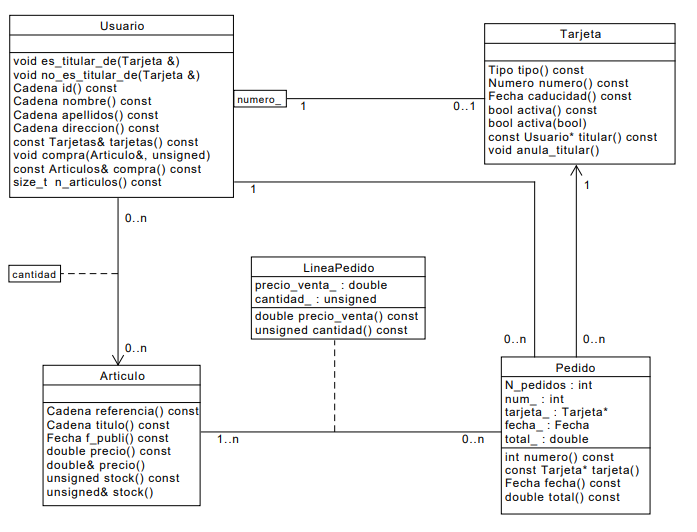
\includegraphics[width=\textwidth]{Pics/P3_1.png}
  \end{center}
  \caption{Diagrama de clases de la práctica 3.}
\end{figure}

En esta práctica haremos modificaciones en la clase Número para poder trabajar con predicados y objetos a funciones. Además crearemos nuevas clases como Pedido y LineaPedido y las clases de asociacion Pedido\_Articulo, Usuario\_Pedido.
\newpage
\section{Modificación de la clase Numero}
  En la práctica anterior definimos e implementamos dos métodos para quitar los espacios y obtener la longitud del Numero (ambos métodos privados de la clase).

Ahora vamos a reimplementar el método de quitar los espacios mediante el uso de dos algoritmos de la STL \texttt{remove\_if()} y \texttt{find\_if()}, donde ambos reciben un predicado.

Para el método \texttt{remove\_if()} vamos a declarar un objeto a función llamado \textbf{Numero::EsBlanco} o bien hacer uso de una función Lambda para detectar si el caracter es un espacio o no mediante el método \texttt{isspace()}.

Por otro lado, para el método \texttt{find\_if()} vamos a hacer uso de un objeto a función llamado \textbf{Numero::EsDigito} para detectar dígitos, y combínelo con el adaptador de negación unaria disponible en \texttt{<functional>} para detectar
caracteres que no sean dígitos. Esta clase la tenemos que definir como miembro público de la clase Numero.

Todo esto se realiza en el constructor de la clase Numero por lo que los métodos anteriores (longitud y eliminar\_espacios) desaparecen.
\subsection{Numero.hpp}
\begin{minted}[breaklines]{C++}
  class Numero{
  public:
    // tipos de excepciones
    typedef enum{ LONGITUD,DIGITOS,NO_VALIDO} Razon;
    Numero(const Cadena &);
  
    // operador de conversion a const char*
    inline operator const char *() const{
        return numero_.operator const char *();}
    // sobrecarga del operador < para comparar numeros
    friend bool operator<(const Numero &, const Numero &);
    // clase de la excepcion
    class Incorrecto{
      Razon razon_;
    public:
      Incorrecto(const Razon &r) : razon_(r){};
      const Razon &razon() const { return razon_; }
    };
    // Objeto a función para comprobar si son digitos
    class EsDigito : public std::unary_function<char, bool>{
    public:
      bool operator()(char caracter) const { return isdigit(caracter); }
    };
  private:
    Cadena numero_;
  };
\end{minted}

\subsection{Numero.cpp}
\begin{minted}[breaklines]{C++}
Numero::Numero(const Cadena& numero){
  Cadena aux(numero);
  //hacemos uso de los predicados para los algoritmos remove_if, find_if
  //Eliminamos los espacios del numero
  auto quitaespacios = std::remove_if(aux.begin(),aux.end(),[](char c){
    return isspace(c);});
  //Modificamos el número fisicamente
  if(quitaespacios != aux.end()){
      aux = aux.substr(0, quitaespacios-aux.begin());
  }
  //negamos que sea un digito y buscamos caracteres que no sean digitos
  auto j = std::find_if(aux.begin(),aux.end(),not_fn(EsDigito()));

  if(j!=aux.end()) //si encuentra un caracter no numérico, excepción
      throw Incorrecto(Razon::DIGITOS); 

  if(aux.length()>19 || aux.length() < 13 || aux.length() == 0)
      throw Incorrecto(Razon::LONGITUD);

  //comprobamos que sea correcto
  if(!luhn(aux))
      throw Incorrecto(Razon::NO_VALIDO);

  //actualizamos el numero sin espacios ni caracteres no numéricos
  numero_ = aux;
}
\end{minted}

\newpage
\section{Clase Pedido}
  Vamos a crear una clase nueva llamada Pedido la cual va a contener información sobre los pedidos que van a poder realizar los Usuarios.

Como vemos en el diagrama contiene 5 atributos:
\begin{itemize}
  \item Dos tipos enteros uno para el número total de pedidos (N\_pedidos) y otro para el número del pedido que se va a realizar.
  \item Un tipo puntero a Tarjeta, que es la tarjeta con la que se realiza el pago.
  \item Un tipo Fecha que es la fecha del pedido.
  \item Un tipo double que es el precio total del pedido.
\end{itemize}

El constructor va recibir los siguientes parámetros:
\begin{itemize}
  \item La asociación entre Usuario y Pedido (Usuario\_Pedido).
  \item La asociación entre Articulo y Pedido (Articulo\_Pedido).
  \item El Usuario que realiza el Pedido.
  \item La Tarjeta con la que se realiza el pago.
  \item La Fecha del pedido, por defecto es la del sistema.
\end{itemize}

Cuando se va a crear el pedido vamos a llamar a los métodos correspondientes para que se relacionen la clases entre sí, estas estarán en las clases de asociación previamente comentadas.

Vamos a crear la clase de excepción \textbf{Pedido::Vacio} para evitar así crear pedidos vacíos. Esta clase tiene un atributo que es un puntero al usuario que realiza el pedido, un constructor que recibe el usuario y un método observador usuario que lo devuelve.

También vamos a declarar la clase de excepción \textbf{Pedido::Impostor}, para poder comprobar que el Usuario que realiza el pedido es el mismo que el titular de la Tarjeta. Al igual que en la clase de excepción anterior, el atributo almacena un puntero al usuario, el constructor recibe el usuario y el observador lo devuelve.

Como los articulos tienen un stock definido, puede ser que algún articulo del carrito supere la cantidad de existencias por eso vamos a crear la clase de excepción \textbf{Pedido::SinStock} que lanzará la excepción y se eliminará el contenido del carrito. Esta clase de excepción consta de un atributo de tipo puntero a Articulo, un constructor que recibe el primer artículo del carrito sin existencias suficientes y un método observador articulo que lo devuelve.

No podemos realizar un pago de un pedido con una tarjeta que esté caducada por tanto, en el construtor de Pedido vamos a lanzar la excepción \textbf{Tarjeta::Caducada} cuando la fecha de caducidad de la tarjeta sea menor a la fecha del pedido. Si la Tarjeta está desactivada vamos a lanzar la excepción \textbf{Tarjeta::Desactivada}. Esta última es una clase de excepción vacía que habrá que añadir a la clase Tarjeta definida en la práctica anterior.

También contamos con varios métodos observadores: \texttt{numero()}, \texttt{tarjeta()}, \texttt{fecha()}, \texttt{total()} y \texttt{n\_total\_pedidos()} que devuelven los atributos correspondientes.

Por último, realizaremos una sobrecargar del operador de inserción en flujo (\texttt{operator <<}) para imprimir un Pedido por pantalla.\\
Mediante el formato:

\texttt{\\
Núm. pedido: 1\\
Fecha: jueves 10 de marzo de 2016\\
Pagado con: VISA n.º: 4539451203987356\\
Importe: 149,95 €\\
}
\subsection{Pedido.hpp}
\begin{minted}[breaklines]{C++}
#ifndef _PEDIDO_HPP_
#define _PEDIDO_HPP_

//Inclusión de librerias y cabeceras
#include "tarjeta.hpp"
#include "usuario.hpp"
#include "articulo.hpp"
#include "usuario-pedido.hpp"
#include "pedido-articulo.hpp"

//Declaraciones adelantadas
class Tarjeta;
class Pedido_Articulo;
class Usuario_Pedido;

class Pedido{
  public:
    Pedido(Usuario_Pedido& ,Pedido_Articulo& ,Usuario& ,const Tarjeta& ,const Fecha& f=Fecha());
    
    //Observadores de la clase
    int numero()const noexcept {return num_;}
    const Tarjeta* tarjeta()const noexcept{return tarjeta_;}
    const Fecha& fecha()const noexcept{return f_pedido_;}
    double total()const noexcept{return importe_Total_;}
    static int n_total_pedidos() noexcept{return n_pedidos_;}

    //clase de la excepcion vacio
    class Vacio{
        Usuario* user_;
      public:
        Vacio(Usuario* user):user_(user){}
        Usuario& usuario()const{return *user_;}
    };

    //clase de la excepción Impostor
    class Impostor{
        Usuario* user_;
      public:
        Impostor(Usuario* user):user_(user){}
        Usuario& usuario()const{return *user_;}
    };

    //clase de la excepción SinStock
    class SinStock{
        Articulo* articulo_;
      public:
        SinStock(Articulo* articulo):articulo_(articulo){}
        Articulo& articulo()const{return *articulo_;}
    };

  private:
    int num_;
    const Tarjeta* tarjeta_;
    Fecha f_pedido_;
    double importe_Total_;
    static int n_pedidos_;
};

//Sobrecarga del operador de flujo
std::ostream& operator <<(std::ostream& ,const Pedido& )noexcept;

#endif //!PEDIDO.HPP
\end{minted}
\subsection{Pedido.cpp}
\begin{minted}[breaklines]{C++}
#include "pedido.hpp"

//Inicializamod la variable static
int Pedido::n_pedidos_ = 0;

//Constructor
Pedido::Pedido(Usuario_Pedido& up,Pedido_Articulo& pa,Usuario& u, const Tarjeta& t,const Fecha& f):num_(n_pedidos_+1),tarjeta_(&t),f_pedido_(f),importe_Total_(0.0){
  //Vamos a comprobar todas la excepciones del constructor de pedido
  //Si el usuario no tiene una compra realizada, el pedido está vacio
  if(u.compra().empty()) throw Pedido::Vacio(&u);

  //Si el usuario es otro al que realiza la compra, excepción
  if(t.titular()!=&u) throw Pedido::Impostor(&u);

  //Si la tarjeta está caducada o desactivada, excepción
  if(t.caducidad() < f_pedido_) 	throw Tarjeta::Caducada(t.caducidad());

  if(!t.activa()) throw Tarjeta::Desactivada();
  //Si no hay stock del articulo, excepción
  for(auto i : u.compra()){
    if(i.first->stock()<i.second){
      u.vaciar_carro();
      throw Pedido::SinStock(i.first);
    }
  }
  //Creamos la asociación entre las clases una vez que todo está correcto
  /*Asociación Usuario-Pedido*/
  up.asocia(*this,u);
  //actualizamos el importe del pedido y pedimos el articulo
  for(auto& i : u.compra()){
    //importe_Total_ += precio_articulo * cantidad del mismo.
    importe_Total_ += i.first->precio() * i.second;
    pa.pedir((*i.first),*this,i.first->precio(),i.second);

    //restamos el stock del articulo que se ha pedido
    i.first->stock() -= i.second; //sobrecarga del operador -=
  }
  //Aumentamos el numero de pedidos y vaciamos el carro del usuario
  u.vaciar_carro();
  n_pedidos_++;
}

//Insersión en flujo
std::ostream& operator <<(std::ostream& output , const Pedido& ped)noexcept{
  output<<"Núm. pedido: "<<ped.numero()<<std::endl
    <<"Fecha:\t"<<ped.fecha()<<std::endl
    <<"Pagado con: "<<ped.tarjeta()->tipo()<<" n.º: "<<ped.tarjeta()->numero()<<std::endl
    <<"Importe: "<<std::fixed<<std::setprecision(2)<<ped.total()<<" €"<<std::endl;
  return output;
}
  
\end{minted}


\newpage

\section{Clase asociación Articulo\_Pedido}
  Como vemos en el diagrama de clase la asociación entre las clases Articulo y Pedido tiene una clase de asociación llamada LineaPedido.

Esta clase la vamos a incluir en el fichero de cabecera Articulo\_Pedido.hpp y la implementaremos en el fichero Articulo\_Pedido.cpp.

\subsection{Clase LineaPedido}
La clase LineaPedido va a contener algunos atributos y métodos necesarios para que la relación bidireccional entre Articulo y Pedido se lleve a cabo. Cuenta con los atributos:
\begin{itemize}
  \item Un tipo double que es el precio de la venta (precio\_venta).
  \item Un entero sin signo que almacena la cantidad de ariculos (cantidad\_).
\end{itemize}

Teniendo claro esto, un objeto de LineaPedido se crea mediante estos dos atributos que se le pasarán como parámetros, los cuales tendrán valores por omisión, (0.0) para el precio de venta y 1 para la cantidad.

Declararemos el constructor como \texttt{explicit} debido a que no se permiten conversiones implícitas.

La clase LineaPedido tendrá un par de métodos observadores llamados \texttt{precio\_venta()} y \texttt{cantidad()}.

Finalmente, declararemos una sobrecarga del operador de inserción en flujo \texttt{operator <<} para imprimir un objeto LineaPedido. \textbf{Ejemplo: 35,20␣€ TAB 3}.
\newpage
\subsection{Clase de asociación Articulo\_Pedido}
Como hemos comentado anteriormente esta clase representará la relación bidireccional entre las clases Articulo y Pedido, por tanto, va a contener todos los métodos imprescindibles para que dicha relación se lleve a cabo.

Si nos fijamos en el diagrama de clases, vemos que la relación entre ambas clases es 1..N - M, por tanto, la clase va a tener dos atributos que serán dos diccionarios:
\begin{itemize}
  \item \underbar{Relación Articulo - Pedido:} Este diccionario será del tipo\\ \texttt{std::map<Pedido*,ItemsPedido,OrdenaPedidos>}, donde \textbf{ItemsPedido} es un método público de la clase definido como otro diccionario:\\ \texttt{std::map<Articulo*,LineaPedido,OrdenaArticulos>}. \textbf{OrdenaPedidos} y \textbf{OrdenaArticulos} serán dos  tipos públicos definidos como dos clases anidadas. Se trata de dos clases de objetos función para ordenar ascendentemente los pedidos y artículos por número y referencia, respectivamente, dentro de los diccionarios.

  \item \underbar{Relación Pedido - Articulo:} Se representará por un diccionario del tipo\\ \texttt{std::map<Articulo*,Pedidos,OrdenaArticulos>}, donde Pedidos será un tipo público definido como \texttt{std::map<Pedido*,LineaPedido,OrdenaPedidos>}.
\end{itemize}

NO es necesario definir los constructores.

Como tenemos varios diccionarios para la creación de estos enlaces vamos a declarar varios métodos para insertar los elementos en los diccionarios correspondientes, para ello contamos con el método \texttt{pedir()} que recibe por parámetro el Articulo, Pedido, el precio y la cantidad (por defecto es 1). Tenemos que realizar una sobrecarga de dicho método invirtiendo el orden del Articulo y Pedido, este método es de tipo void.

Contamos con un observador llamado \texttt{detalle()} que dado un Pedido, nos devuelve el diccionario de los articulos de un pedido, es decir \textbf{ItemsPedido} mediante una referencia constante, ya que la multiplicidad es ``1..N''.

También contamos con un observador que nos devuelve los pedidos \textbf{Pedidos}, que ha realizado un Articulo, este método se llamará \texttt{ventas()}. Aquí devolvemos una copia debido a que la multiplicidad es ``N'' y por tanto, pueden haber objetos que no estén instanciados.

Realizaremos dos sobrecargas del operador de inserción en flujo \texttt{operator <<} para los tipos de datos \textbf{Pedido\_Articulo::ItemsPedido} y\\ \textbf{Pedido\_Articulo::Pedidos}. El primero mostrará los detalles del pedido y, además, el importe total. El segundo mostrará precio, cantidad y fecha de cada venta, así como el importe total de las ventas del artículo y el número de ejemplares vendidos.
\newpage
\subsubsection*{Ejemplo de salida de los detalles de un pedido:}
\begin{center}
  \begin{verbatim}
PVP   Cantidad  Artículo
==================================================================
35,20 € 2 [100] "Programación Orientada a Objetos"
29,95 € 1 [110] "Fundamentos de C++"
==================================================================
Total 100,35 €
  \end{verbatim}
\end{center}
\subsubsection{Ejemplo de salida de pedidos:}
\begin{center}
  \begin{verbatim}
[Pedidos: 3]
==================================================================
PVP   Cantidad  Fecha de venta
==================================================================
39,95 € 2 miércoles 19 de abril de 2017
34,90 € 1 jueves 20 de abril de 2017
34,90 € 1 lunes 5 de abril de 2010
==================================================================
149,70 € 4
  \end{verbatim}
\end{center}

También tendremos un método llamado \texttt{mostrarDetallePedidos()} imprimirá en el flujo de salida proporcionado el detalle de todos los pedidos realizados hasta la fecha, así como el importe de todas las ventas.
\subsubsection*{Ejemplo de salida de mostrarDetallePedidos:}
\begin{center}
  \begin{verbatim}
Pedido núm. 1
Cliente: lucas Fecha: viernes 10 de marzo de 2017

detalle de ese pedido, como en ejemplo anterior
Resto de los pedidos ...

TOTAL VENTAS 981,60 €
  \end{verbatim}
\end{center}

Por último, un método llamado \texttt{mostrarVentasArticulos()} visualizará en el flujo de salida proporcionado todas las ventas agrupadas por artículos.\subsubsection*{Ejemplo de salida de mostrarVentasArticulos:}
\begin{center}
  \begin{verbatim}
Ventas de [110] "Fundamentos de C++"
pedidos de ese artículo, como en ejemplo anterior
Resto de los artículos vendidos ...
  \end{verbatim}
\end{center}
\subsection{Articulo\_Pedido.hpp}
\begin{minted}[breaklines]{C++}
#ifndef PEDIDO_ARTICULO_HPP
#define PEDIDO_ARTICULO_HPP

//Inclusión de librerias y cabeceras
#include "pedido.hpp"
#include "articulo.hpp"
#include <map>

//Contendrá LineaPedido
class LineaPedido{
  public:
    explicit LineaPedido(double precio = 0.0, unsigned cant=1)
        :precio_venta_(precio),cantidad_venta_(cant){}
    //Métodos observadores de la clase
    double precio_venta()const noexcept{return precio_venta_;}
    unsigned cantidad()const noexcept{return cantidad_venta_;}
  private:
    double precio_venta_;
    unsigned cantidad_venta_;
};
//Operador de inserción en flujo de LineaPedido
std::ostream& operator <<(std::ostream& , const LineaPedido&)noexcept;

//Clase de asociación entre Pedido - Articulo
class Pedido_Articulo{
  public:
  struct OrdenaArticulos{
    bool operator () (const Articulo*, const Articulo* )const;
  };

  struct OrdenaPedidos{
    bool operator()(const Pedido* , const Pedido* )const;
  };
    //Diccionarios de la clase Pedido - Articulo
    typedef std::map<Articulo*,LineaPedido,OrdenaArticulos>ItemsPedido;
    typedef std::map<Pedido*,ItemsPedido,OrdenaPedidos> PedidoArticulo;
    //Diccionarios de la clase Articulo - Pedido
    typedef std::map<Pedido*,LineaPedido,OrdenaPedidos>Pedidos;
    typedef std::map<Articulo*,Pedidos,OrdenaArticulos> ArticuloPedido;
    //Creacion de enlaces
    void pedir(Pedido&,Articulo&,double,unsigned cantidad = 1); //directa
    void pedir(Articulo&,Pedido&,double,unsigned cantidad = 1); //inversa
    //observador que devuelve los articulos de un pedido
    const ItemsPedido& detalle(Pedido& )const;
    //observador que devuelve los pedidos de un articulo
    Pedidos ventas(Articulo& )const;
    //Métodos que imprimen detalles de los pedidos y ventas
    std::ostream& mostrarDetallePedidos(std::ostream&)const noexcept;
    std::ostream& mostrarVentasArticulos(std::ostream&)const noexcept;
  private:
    //Diccionarios de la clase
    PedidoArticulo pedido_articulo_; //directa
    ArticuloPedido articulo_pedido_; //inversa
};

//Sobrecarga de los operadores de inserción en flujo
std::ostream& operator << (std::ostream& , const Pedido_Articulo::ItemsPedido&)noexcept;
std::ostream& operator << (std::ostream& , const Pedido_Articulo::Pedidos&) noexcept;
#endif // !PEDIDO_ARTICULO_HPP

\end{minted}

\subsection{Articulo\_Pedido.cpp}
\begin{minted}[breaklines]{C++}
//Implementación de la clase LineaPedido
std::ostream& operator <<(std::ostream& output , const LineaPedido& lp)noexcept{
  return output << std::fixed<<std::setprecision(2)<<lp.precio_venta()<<" €\t" <<lp.cantidad();
}

//Implementación de la clase Pedido_Articulo
bool Pedido_Articulo::OrdenaArticulos::operator()(const Articulo* a1, const Articulo* a2) const{ return (a1->referencia() < a2->referencia()); }  

bool Pedido_Articulo::OrdenaPedidos::operator()(const Pedido* p1, const Pedido* p2)const{ return (p1->numero() < p2->numero()); }

void Pedido_Articulo::pedir(Pedido& p, Articulo& a, double precio, unsigned cant){
    //Creamos una LineaPedido nueva
    LineaPedido lp(precio,cant);
    //creamos los enlaces directa e inversamente
    pedido_articulo_[&p].insert(std::make_pair(&a,lp));
    articulo_pedido_[&a].insert(std::make_pair(&p,lp));
}

void Pedido_Articulo::pedir(Articulo& a,Pedido& p,double precio,unsigned cant){
    pedir(p,a,precio,cant);//Delegamos en el método anterior
}

const Pedido_Articulo::ItemsPedido& Pedido_Articulo::detalle(Pedido& p)const{
  //Como siempre habrá como minimo un articulo en el pedido, devolvemos directamente los articulos de dicho pedido.
  return pedido_articulo_.find(&p)->second;
}

Pedido_Articulo::Pedidos Pedido_Articulo::ventas(Articulo& a)const{
    //buscamos el articulo, para ver si tiene un pedido asignado o no
    auto i = articulo_pedido_.find(&a);
    if(i!=articulo_pedido_.end())return i->second; //devolvemos pedidos
    else{//no hay pedido asignado, devolvemos conjunto vacio.
        Pedido_Articulo::Pedidos PedidoVacio;
        return PedidoVacio;
    }
}

//Implementación de los métodos de inserción en flujo
std::ostream& operator << (std::ostream& output,const Pedido_Articulo::ItemsPedido& IP)noexcept{
    //nos creamos una variable local para obtener el precio total
    double total = 0.;
    output <<"PVP\t Cantidad\t Artículo"<<std::endl
    << std::setw(65)<<std::setfill('=')<<' '<<std::endl; //formato
    //insertamos el pedido
    for(auto& i :IP){
        total += i.second.precio_venta()*i.second.cantidad();
        output<<std::fixed<<std::setprecision(2)<<i.second.precio_venta()<<" € "
        <<i.second.cantidad()<<"\t"
        <<"["<<i.first->referencia()<<"] \""<<i.first->titulo()<<"\""<<std::endl;
    }
    output <<  std::setw(65)<<std::setfill('=')<<' '<<std::endl
    <<"Total "<<std::fixed<<std::setprecision(2)<<total<<" €";
    return output; //devolvemos el flujo de salida
}



std::ostream& operator <<(std::ostream& output,const Pedido_Articulo::Pedidos& Ped)noexcept{
    //Nos creamos una variable local para obtener el precio total y el numero de pedidos
    double total = 0.;
    unsigned npedido =1;
    output<<"[Pedidos: "<<npedido<<"]"<<std::endl
      <<std::setw(65)<<std::setfill('=')<<" "<<std::endl//formato
      <<"PVP \t Cantidad \t Fecha de venta"<<std::endl
      <<std::setw(65)<<std::setfill('=')<<" "<<std::endl;//formato
    for(auto& i : Ped){
    //actualizamos el numero de pedido y el total
      total+=i.second.precio_venta()*i.second.cantidad();
      npedido++;
      output<<i.second.precio_venta()<<" €\t"<<i.second.cantidad()<<"\t"
      <<i.first->fecha()<<std::endl;
    }
    output<<std::setw(65)<<std::setfill('=')<<" "<<std::endl//formato
          <<std::fixed<<std::setprecision(2)<<total<<" €\t "<<npedido<<std::endl;
    return output;
}
std::ostream& Pedido_Articulo::mostrarDetallePedidos(std::ostream& output)const noexcept{
    //Creamos variables locales para alamecenar el numero de pedido y el total de ventas
    double total=0.;
    unsigned npedido=0;
    for(auto& i : pedido_articulo_){
      npedido++;
      output<<"\nPedido núm. "<<npedido<<std::endl
            <<"Cliente: "<< *i.first->tarjeta()->titular()
            <<detalle(*i.first)<<std::endl;
      total += i.first->total();
    }
    output<<"TOTAL VENTAS\t "<<std::fixed<<std::setprecision(2)<<total<<" €"<<std::endl;
    return output;
}
std::ostream& Pedido_Articulo::mostrarVentasArticulos(std::ostream& output)const noexcept{
  for(auto& i : articulo_pedido_){
    output<<"Ventas de ["<<i.first->referencia()<<"] "<<"\""<<i.first->titulo()<<"\"\n"<<ventas(*i.first)<<std::endl;
  }
  return output;
}
\end{minted}
\newpage
\section{Clase de asociación Usuario\_Pedido}
  Si nos fijamos en el diagrama de clases de la práctica vemos que la relación entre las clases Usuario y Pedido es una relación de asociación pero sin atributos de enlace cuya multiplicidad es 1 - N.

Esta clase de asociación va a almacenar dos atributos:
\begin{itemize}
  \item Un diccionario de puntero Usuario a un conjunto de elementos Pedidos (set):
  \begin{center}
    \begin{verbatim}
      typedef std::set<Pedido*>Pedidos;
      typedef std::map<Usuario*,Pedidos>Usuario_Pedido;
    \end{verbatim}
  \end{center}
  \item Un diccionario de puntero Pedido a puntero Usuario.
  \begin{center}
    \begin{verbatim}
      typedef std::map<Pedido*,Usuario*>Pedido_Usuario;
    \end{verbatim}
  \end{center}
\end{itemize}

Vamos a contar con dos métodos llamados \texttt{asocia()} que recibe por parámetro una referencia a Usuario y a Pedido. Debemos de realizar una sobrecarga del método intercambiando el orden de los parámetros.

Por otro lado, tenemos dos métodos observadores:
\begin{itemize}
  \item Método llamado \texttt{pedidos()} que recibe como parámetro una referencia a Usuario y devuelve los Pedidos del mismo. Como puede haber un Usuario sin pedidos devolvemos una copia.
  \item Método llamado \texttt{cliente()} que dado una referencia de un Pedido, este devuelve la dirección de memoria del Usuario que ha hecho el pedido.
\end{itemize}

\subsection{Usuario\_Pedido.hpp}
\begin{minted}[breaklines]{C++}
#ifndef USUARIO_PEDIDO_HPP
#define USUARIO_PEDIDO_HPP
// Incluimos cabeceras
#include "usuario.hpp"
#include "pedido.hpp"

class Usuario_Pedido{
public:
  typedef std::set<Pedido *> Pedidos;
  typedef std::map<Usuario *, Pedidos> UsuarioPedidos;
  typedef std::map<Pedido *, Usuario *> PedidoUsuario;

  void asocia(Usuario &, Pedido &) noexcept;
  void asocia(Pedido &, Usuario &) noexcept;

  // pedidos recibe un Usuario y devuelve los pedidos que éste ha realizado.
  Pedidos pedidos(Usuario &) const noexcept;
  // cliente recibe un Pedido y devuelve la dirección de memoria del usuario que ha hecho el pedido.
  Usuario *cliente(Pedido &) const noexcept;

private:
  UsuarioPedidos usuariopedidos_;
  PedidoUsuario pedidousuario_;
};

#endif //! USUARIO_PEDIDO.HPP
\end{minted}

\subsection{Usuario\_Pedido.cpp}
\begin{minted}[breaklines]{C++}
// Implementación de los métodos de la clase de asociación
void Usuario_Pedido::asocia(Usuario &u, Pedido &p) noexcept{
  usuariopedidos_[&u].insert(&p);
  pedidousuario_[&p] = &u;
}

void Usuario_Pedido::asocia(Pedido &p, Usuario &u) noexcept{
  // delegamos en el método anterior
  asocia(u, p);
}

Usuario_Pedido::Pedidos Usuario_Pedido::pedidos(Usuario &u) const noexcept{
  // comprobamos que existe el usuario
  auto i = usuariopedidos_.find(&u);
  if (i != usuariopedidos_.end())
    return i->second;
  else{
    Usuario_Pedido::Pedidos pedidovacio;
    return pedidovacio;
  }
}

Usuario *Usuario_Pedido::cliente(Pedido &p) const noexcept{
  // devolvemos el usuario de dicho pedido
  return pedidousuario_.find(&p)->second;
}
\end{minted}
